%!TeX root=MemoriaTFG.tex

\chapter{Análisis del proyecto} \label{analisis_proyecto}


Este capítulo recoge toda la información sobre la metodología de desarrollo empleada para el desarrollo del trabajo, los requerimientos  funcionales del proyecto, las restricciones y los objetivos cuantificables que se esperan alcanzar al final del trabajo.

\section{Metodología de desarrollo del proyecto}

Durante la realización de un proyecto es necesario seguir una serie de pautas que permitan la organización, la estructuración y el control del trabajo realizado para procurar seguir una correcta fluidez de desarrollo. Dichas pautas se recogen dentro de los llamados \textbf{\textit{modelos de desarrollo de software}}. Existen distintos tipos de modelos, como por ejemplo el modelo en cascada, el modelo iterativo y el modelo incremental. \\ 

El trabajo realizado para este proyecto ha sido basado en el llamado \textit{modelo de prototipado}, ya que se ha ido implementado, probando y modificando el código y los experimentos a lo largo del desarrollo hasta alcanzar un sistema estable. 

\subsection{El modelo de prototipado}

El \textbf{modelo de prototipado}, también denominado como \textbf{\textit{modelo de desarrollo evolutivo}} o \textbf{\textit{modelo de prototipado incremental}}, se basa en la creación de un (o varios) prototipo del producto final antes de empezar con la implementación del producto. De esta manera es muy sencillo entender cómo será el aspecto y qué características y funcionalidades tendrá el producto final. \\

Tal como aparecen en \cite{modeloPrototipos2}, las características del prototipo son: 

\begin{enumerate}
    \item Es una \textbf{aplicación que funciona}: contiene las funcionalidades desarrolladas a $"$bajo nivel$"$ para que el usuario pueda utilizarlo como si se tratase del producto final y, de esta manera, generar opiniones sobre su funcionamiento.
    \item Se \textbf{crea con rapidez}: debido a que no se tienen que desarrollar las funcionalidades teniendo en cuenta la seguridad, la fiabilidad, la eficacia, u otros aspectos importantes en la implementación, la creación de los prototipos es muy rápida. 
    \item \textbf{Evoluciona} a través de un proceso iterativo:  Con cada prototipo realizado los usuarios lo utilizan y ofrecen una retroalimentación con su experiencia. Cada \textit{feedback} recibido sirve para ajustar las características del prototipo, por lo que cuanto más rápido se reciba dicha respuesta, más rápido se creará el prototipo perfecto con el que se realizará el producto final. 
    \item Tiene un \textbf{coste bajo de desarrollo}: no se deben incorporar servicios costosos ni tener un gran equipo de desarrollo puesto que no se trata del producto final. 
\end{enumerate}

Como bien se menciona en \cite{calameoModeloPrototipado}, \textit{el éxito del uso del prototipo depende de la rapidez y de la frecuencia con la que se reciba el \textbf{feedback} del usuario para hacer cambios y adecuarlos a las necesidades actuales}. Aplicado al proyecto en cuestión, y el usuario final siendo la persona que ha realizado el TFG, 

\begin{itemize}
    \item La \textit{rapidez} es prácticamente inmediata ya que el usuario final y el desarrollador son el mismo.
    \item La \textit{frecuencia} es después de cada experimentación realizada; se valora el prototipo y se aplican las modificaciones necesarias para generar uno nuevo y volver al proceso de experimentación.
\end{itemize}

\subsection{Etapas del modelo de prototipado}

La implementación del software cuando se trata de este tipo de modelo es \textbf{\textit{iterativa}}, ya que se debe diseñar el prototipo, implementarlo y testearlo con usuarios final varias veces hasta tener un prototipo satisfactorio. \\

\begin{figure}[h]
    \centering
    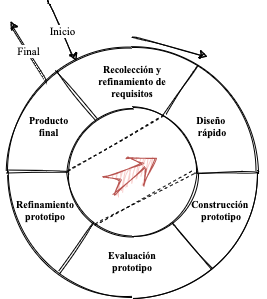
\includegraphics[width=0.3\textwidth]{cap3_analisis_tecnico/images/modelo_prototipado.png}
    \caption{Fases del modelo de prototipado}.
    \label{fig:modelo_prototipado}
\end{figure}

De acuerdo con la definición de \cite{modeloPrototipos1} se ha desarrollado la Fig. ~ \ref{fig:modelo_prototipado} y, cómo se puede apreciar, existen 6 fases en este modelo:

\begin{enumerate}
    \item \textbf{Recolección y refinamiento de requerimientos }: se plantean las características que se desea que tenga el producto final: aspecto, funcionalidad, restricciones, etc. 
    \item \textbf{Diseño rápido}: se diseña el prototipo a partir de las especificaciones ofrecidas.
    \item \textbf{Construcción prototipo}: se implementa el prototipo.
    \item \textbf{Evaluación prototipo}: se evalúa con los usuarios finales.
    \item \textbf{Refinamiento prototipo}: se analiza el \textit{feedback} y si es necesario se hacen cambios en el prototipo. En caso de que esto ocurra, se vuelve a la etapa 2 de diseño.
    \item \textbf{Producto final}: el prototipo ya está listo y se pasa a implementar el producto final. En el caso de este proyecto el producto final es el \textbf{último prototipo} desarrollado que se obtiene al cabo de todo el proceso; es suficiente ya que se trata de una investigación y que, además, dicho prototipo permite conseguir toda la información necesaria para obtener conclusiones válidas del estudio. 
\end{enumerate}



\subsection{Ventajas del modelo de prototipado}
Las ventajas de este modelo son las siguientes \cite{modeloPrototipos1, modeloPrototipos2, ventajasDesventajasPrototipos}: 

\begin{itemize}
    \item \textbf{Útil cuando se conocen los objetivos generales} para el software pero \textbf{no se identifican los requerimientos  detallados} de entrada, procesamiento o salida. Permiten el desarrollo de un sistema a partir de requerimientos  poco claros o cambiantes.
    \item \textbf{No modifica el flujo del ciclo de vida} ya que hasta que se desarrolle un prototipo final no se sale de la etapa de diseño.
    \item \textbf{Aumentan las probabilidades de éxito debido al constante \textit{feedback} que hay sobre el sistema}; esto hace que sea improbable que el producto final no sea el esperado.
    \item \textbf{Reduce el riesgo de construir productos que no satisfagan las necesidades de los usuarios} porque estos están constantemente probándolo y aportando ideas de mejora de usabilidad.
    \item  \textbf{Son más fáciles de abordar con los usuarios finales.} Su uso redunda en una mayor satisfacción del usuario con el producto final, ya que él o ella han participado activamente de su diseño. \textbf{Curva menor de aprendizaje} al comenzar a usar el sistema final. 
    \item \textbf{Permite a todos los involucrados entender bien y mejor el problema antes de la implementación final.}
    \item Se \textbf{reduce el riesgo} o la \textbf{incertidumbre sobre la implementación del software} ya que antes de empezar con el producto final, el prototipo ya estará muy bien estudiado por lo que se conocerán cuáles son las necesidades de implementación.
    \item Como información complementaria a los requerimientos  constituyen un \textbf{gran apoyo a las estimaciones de esfuerzo de todas las áreas}, incluyendo proveedores.
\end{itemize}

\subsection{Desventajas del modelo de prototipado}
Las desventajas de este modelo son las siguientes \cite{modeloPrototipos1, modeloPrototipos2, ventajasDesventajasPrototipos}: 

\begin{itemize}
    \item En la implementación \textbf{el prototipo puede ser modificado y/o ampliado por sus desarrolladores sin consultar} con el cliente, rompiendo así el compromiso de calidad y mantenimiento que tiene con éste.
    \item \textbf{Adoptarlo como el sistema final:} los usuarios y profesionales de sistemas pueden considerar al prototipo como el sistema final cuando aún es incompleto e inadecuado.
    \item \textbf{Los usuarios suelen enfocarse en aspectos “superficiales” del prototipo cuando lo prueban y centrarse menos en su funcionalidad global.} También es posible que se pierda mucho tiempo, innecesariamente, tratando de hacer entender al usuario la finalidad real de los prototipos.
    \item Requiere \textbf{participación activa del usuario} puesto que sus opiniones acerca del prototipo son las que se utilizan para determinar si el prototipo necesita más refinamiento. 
    \end{itemize}

\section{Objetivos}

El objetivo principal de este proyecto es estudiar la capacidad de un agente de aprender a llegar a una casilla en concreto dentro de una matriz después de presentarle con distintas situaciones en las que ha interactuado con el entorno. \\

En cuanto a objetivos más concretos, se quiere:

\begin{enumerate}
    \item Crear un entorno estático y un entorno dinámico para poder presentarle al agente la aleatoriedad de los elementos que percibe y así pueda entrenar bajo condiciones variadas. Por ejemplo, cambio de la meta o del origen, deshabilitación de casillas, etc. 
    
    \item Crear varios modelos para el agente y analizar los datos que genera: media de pasos dados para llegar a la meta, desviación típica de los pasos, error total realizado con los pasos, etc. 
    
    \item Encontrar una conFig. ~ción de ANN
    \begin{enumerate}
        \item Con un mínimo de 10 capas ya que es más probable que el algoritmo converja en una solución. 
        \item Que permita alcanzar una solución con una desviación típica \textit{menor a 3}, porque de lo contrario significaría que el agente no ha llegado a aprender correctamente, es decir, no se ha llegado a una solución.  
    \end{enumerate}
\end{enumerate}


\section{Requerimientos funcionales}

Este proyecto no consta de requerimientos funcionales ya que el sistema no se espera que tenga unos resultados en concreto ni ofrezca un servicio en particular, sino que se trata de una \textbf{experimentación} con la que se llegará a unas conclusiones al cabo de su realización; por lo que, a priori, no es sencillo predecir qué resultados se obtendrán. 
\section{Requerimientos no funcionales}

En cuanto a los requerimientos  funcionales, se tiene: 

\begin{enumerate} \label{requerimientos}
    \item \textbf{RF01}: El proyecto debe hacer uso del \textbf{aprendizaje por refuerzo} para el desarrollo del agente inteligente.
    \item \textbf{RF02}: El proyecto debe implementar el entorno del problema mediante la librería \textit{Gym} de OpenAI \cite{gymDocumentation}.
    \item \textbf{RF03}: El proyecto debe tener el modelo del agente implementado con una \textbf{red neuronal} (\textbf{ANN}).
\end{enumerate}

\section{Herramientas utilizadas para el desarrollo}

En este apartado se detallarán los medios utilizados para la implementación de este proyecto: el lenguaje empleado, las tecnologías, las herramientas y las librerías. 
\subsection{Lenguaje de programación} 

En la actualidad hay un total de 16 lenguajes distintos para el desarrollo de programas de inteligencia artificial \cite{wikiAILanguages}. Para poder elegir un lenguaje es necesario analizar las características y las ventajas de cada uno de ellos y, junto con los requerimientos del proyecto, decidir qué lenguaje es el que mejor se adapta al problema. \\

Debido al elevado número de opciones, se han ido descartando hasta quedar con los más empleados en los últimos años: \textbf{\textit{R}} y \textbf{\textit{Python}}. \\

\textbf{R} es altamente enfocado a la estadística, trato de datos, análisis numéricos y, por supuesto, el Aprendizaje Máquina. \\

\textbf{Python}, por otro lado, se usa en una multitud de ámbitos y consta de una gran comunidad y un gran nombre de librerías. \\

Para la implementación del proyecto se ha elegido el lenguaje \textbf{Python} ya que:

\begin{itemize}
    \item Es \textbf{\textit{fácil de utilizar}} y el código resultante es \textbf{\textit{muy comprensible}}.
    \item \textbf{\textit{Gran número de librerías}} que implementan partes de código necesarios y que, además, supondría una carga añadida si fuese necesario programarlo. En la siguiente sección se concretarán las librerías empleadas. El uso de una librería en concreto, la de Tensorflow, es el motivo principal por el que se ha elegido emplear Python ya que se proporciona una API específica; con R, las bibliotecas son de terceros. 
    \item \textbf{\textit{Comunidad extensa}} y muy implicada, por lo que muchas dudas que puedan surgir a la hora de la implementación es probable que ya esté resuelta si se busca.
\end{itemize}

\subsection{Librerías} 

En el desarrollo de los distintos elementos que componen el proyecto se han utilizado librerías específicas que contienen funciones que facilitan su implementación. A continuación se enumeran las librerías empleadas para cada uno de estos elementos: el \textit{entorno}, el \textit{agente} y los \textit{resultados gráficos}. 

\subsubsection{Librerías para el entorno}

Uno de los requerimientos  de este proyecto era emplear \textit{\textbf{Gym}} \cite{gymDocumentation}, una librería desarrollada por OpenAI que proporciona herramientas para la creación de los entornos empleados en el aprendizaje por refuerzo. \\

Las herramientas de las que dispone \textit{Gym} son empleadas para

\begin{enumerate}
    \item Definir el entorno en el que se encuentra el problema.
    \item Obtener las observaciones y las recompensas obtenidas de una interacción entre agente-entorno \ref{fig:gym_ML}; éstas serán las que determinarán el aprendizaje del agente ya que son indicadores de su comportamiento. Un ejemplo de observación sería: \textit{el agente está a 3 pasos de la meta}. 
\end{enumerate}

Dentro de la librería existen diferentes entornos ya desarrollados y clasificados por el \textit{tipo de problema que se desea resolver}:  \textbf{classic control/toy text}, \textbf{algorithmic}, \textbf{atari}, y  \textbf{2D \& 3D robots} \cite{gymDocumentation}. En el caso de este proyecto, no se ha utilizado ninguna de estas plantillas de entornos, sino que se ha implementado usando como base la clase principal de \texttt{Env} que se encuentra en \textit{Gym}.  \\

Se ha utilizado la última versión \textbf{0.17.1}.

\subsubsection{Librerías para el agente}

Por otro lado, para poder implementar la red neurona, es decir, el agente inteligente, se han utilizado las librerías:

\begin{enumerate}
    \item \textbf{\textit{Tensorflow}} (v. 2.0.0): es una biblioteca de código abierto para \textit{aprendizaje automático}; a través de ésta se pueden desarrollar sistemas capaces de construir y entrenar redes neuronales para detectar y descifrar patrones y correlaciones \cite{tensorflowWikipedia}. Los elementos mediantes los cuales se construyen los sistemas son los llamados \textit{\textbf{tensors}}, estructuras multidimensionales de datos. 
    \item \textbf{\textit{Keras}} (v. 2.3.1): \textit{framework} enfocado al \textit{aprendizaje profundo} (es un tipo de aprendizaje en el que se utilizan redes neuronales de un tamaño considerable, como sería por ejemplo una red de 50 capas con 100 neuronas cada una). Se trata de una API a alto nivel (es decir, es sencilla de emplear y de entender) para las funciones de \textit{Tensorflow}. Los elementos básicos que se tratan en esta biblioteca son las \textbf{capas} (el término en inglés \textit{layers}, son agrupaciones de \textit{tensors}) y los \textbf{modelos}. Los modelos se corresponden, en definitiva, a la red neuronal que se construye, y las operaciones que ofrece dicha librería sirven para realizar el entreno de la red y las posteriores predicciones. 
\end{enumerate}

\subsubsection{Librerías para los resultados gráficos}

Para la representación de los datos y la creación de los gráficos se ha empleado la librería \textbf{\textit{matplotlib}}. Mediante dicha librería es posible 

\begin{itemize}
    \item \textbf{Crear visualizaciones estáticas}; existen muchísimas opciones para producir representaciones \cite{matplotlibGallery}, entre ellas: 
    \begin{itemize}
        \item Líneas, barras y marcadores
        \item Imágenes, contornos y campos
        \item Ejes y Fig. ~s
        \item Elementos estadísticos
        \item Diagramas de tarta y polares
    \end{itemize}
    \item \textbf{Crear visualizaciones dinámicas}, ya que trabaja con distintos \textit{toolkits} de interfaz de usuario (wxpython, tkinter, qt4, gtk, y macosx) \cite{matplotlibUserEvents}; esto posibilitan las interacciones por teclado y ratón, por ejemplo para poder ampliar Fig. ~s. 
\end{itemize}

Se ha utilizado la última versión \textbf{3.1.1}.

\subsubsection{Librerías comunes}

Por último, se ha utilizado las librerías de \textbf{\textit{NumPy}} y \textbf{\textit{Pandas}} para el trato de los datos. 

\begin{itemize}
    \item \textbf{Numpy}: Librería fundamental en la computación científica dentro de Python \cite{numpyDoc}. \\

    Proporciona estructuras del \textbf{tipo multidimensional} (\textit{arrays} y elementos derivados tales como las matrices) y un conjunto de rutinas para operaciones rápidas sobre los arrays, entre las cuales se encuentran las \textbf{matemáticas}, las \textbf{lógicas}, la \textbf{manipulación de las estructuras}, la \textbf{ordenación} y \textbf{selección} de los elementos, la \textbf{entrada/salida} de los elementos, aplicaciones de \textbf{álgebra lineal} y operaciones \textbf{estadísticas} básicas sobre los elementos, y muchas más. \\

    Se ha utilizado la versión \textbf{1.17.4}.
    \item \textbf{Pandas}: Librería que proporciona \textbf{estructuras de datos} (\textit{sencillas} y de \textit{alto rendimiento}) y herramientas para el análisis de datos dentro de Python \cite{pandasDoc}. \\

    Las estructuras de datos son \textbf{rápidas}, \textbf{flexibles} y \textbf{expresivas} y han sido diseñadas con el fin de facilitar el trabajo con datos de tipo \textit{relacional} y \textit{con etiquetas}. Entre las fortalezas de esta librería destacan: 

    \begin{itemize}
    \item \textbf{Facilidad de tratar y adaptar} las estructuras con datos que faltan (NaN), tanto los datos de punto flotante como los que no lo son. 
    \item \textbf{Manipulación sencilla de las dimensiones de los datos} (agregación y eliminación de columnas).
    \item \textbf{Alineamiento de datos automáticos o explícitos}. Los objetos se pueden alinear explícitamente por una serie de etiquetas, o el usuario puede omitir las etiquetas y dejar que las propias estructuras alineen los datos. 
    \item \textbf{Fácil conversión de estructuras de \textit{Python} y \textit{NumPy} a estructuras \textit{pandas}.}
    \item \textbf{Conjunto de operaciones flexibles para aplicar las técnicas de \textit{split-apply-combine}} a los conjuntos de datos; \textit{split} se refiere a la separación de los datos siguiendo un criterio en concreto, \textit{apply} a la aplicación de una función de manera independiente a grupos de datos, y \textit{combine} a la agrupación de los resultados en una única estructura de datos \cite{pandasSplitApplyCombine}.
    \item \textbf{Herramientas de entrada/salida} para el trato de ficheros CSV, Excel, bases de datos, y guardado en formato HDF5. 
\end{itemize}

    Se ha utilizado la última versión \textbf{1.1.2}.

\end{itemize}

\subsection{Software y otros elementos} 

En cuanto a los programas utilizados, se ha empleado el programa \textbf{PyCharm} de JetBrains ya que es en IDE intuitivo, fácil de usar, con integración de GIT, visualización de gráficos, visualización de bases de datos, sencillo proceso para debuggear el código, etc. \\

También se ha empleado la herramienta \textbf{Git} para el control de versiones del proyecto. \\


En este capítulo se ha descrito \textit{la metodología} abordada para el desarrollo del proyecto, se han enumerado los distintos \textit{requerimientos } y \textit{objetivos} planteados y se han explicado las diferentes \textit{herramientas} empleadas en la implementación, desde el lenguaje elegido hasta las distintas librerías empleadas. 